
\de{ĐỀ THI HỌC KỲ II NĂM HỌC 2022-2023}{THPT Trần Quốc Tuấn - Kon Tum}
\begin{center}
	\textbf{PHẦN 1 - TRẮC NGHIỆM}
\end{center}
\Opensolutionfile{ans}[ans/ans]

\begin{ex}%[0X2Y2-1]%[Dự án đề kiểm tra HKII NH22-23 - Lê Hùng Thắng]%[THPT Trần Quốc Tuấn - Kon Tum]%Câu 1
Có bao nhiêu cách xếp $5$ học sinh thành một hàng ngang?
\choice
{$25$}
{$20$}
{\True $120$}
{$5$}
\loigiai{
Số cách xếp $5$ học sinh thành hàng ngang là $5!=120$ cách.}
\end{ex}

\begin{ex}%[0H4Y2-1]%[Dự án đề kiểm tra HKII NH22-23 - Lê Hùng Thắng]%[THPT Trần Quốc Tuấn - Kon Tum]%Câu 2
Cho đường tròn $(C)$ có phương trình: $\left(x-1\right)^2+\left(y-2\right)^2=9$. Tìm tọa độ tâm và bán kính của đường tròn $(C)$.
\choice
{\True Đường tròn $(C)$ có tâm $ I\left(1;2\right)$ và bán kính $ R=3$}
{Đường tròn $(C)$ có tâm $ I\left(-1;-2\right)$ và bán kính $ R=9$}
{Đường tròn $(C)$ có tâm $ I\left(1;2\right)$ và bán kính $ R=9$}
{Đường tròn $(C)$ có tâm $ I\left(-1;-2\right)$ và bán kính $ R=3$}
\loigiai{
Đường tròn $(C)$ có tâm $ I\left(1;2\right)$ và bán kính $ R=3$.}
\end{ex}

\begin{ex}%[0X1B1-3]%[Dự án đề kiểm tra HKII NH22-23 - Lê Hùng Thắng]%[THPT Trần Quốc Tuấn - Kon Tum]%Câu 3
Dân số tỉnh Kon Tum năm 2020 là $a=561742$ người, với độ chính xác $d=200$. Số quy tròn của $a$ là
\choice
{$561000$}
{$561800$}
{\True $562000$}
{$561700$}
\loigiai{
Ta có $\overline{a}=a\pm d=567142 \pm 200$.\\
Suy ra số quy tròn của $a$ là $567100$.}
\end{ex}

\begin{ex}%[0H3Y1-3]%[Dự án đề kiểm tra HKII NH22-23 - Lê Hùng Thắng]%[THPT Trần Quốc Tuấn - Kon Tum]%Câu 4
\immini [thm]{	Trong mặt phẳng $Oxy$, cho điểm $A$ như hình vẽ. Tọa độ véc-tơ $\overrightarrow{OA}$ là
	\choice
	{$\overrightarrow{OA}=(-4;-3)$}
	{$\overrightarrow{OA}=(-4;-3)$}
	{\True $\overrightarrow{OA}=(-4;3)$}
	{$\overrightarrow{OA}=(4;3)$}
}
{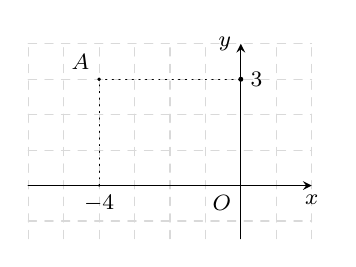
\begin{tikzpicture}[scale=0.45,>=stealth, font=\footnotesize, line join=round, line cap=round]
		\def\a{1} \def\b{-4} \def\c{3} % Hệ số
		\def\xmin{-6} \def\xmax{2}
		\def\ymin{-1.5} \def\ymax{4}	
		\draw[color=gray!30,dashed] (\xmin,\ymin) grid (\xmax,\ymax);
		\draw[->] (\xmin,0)--(\xmax,0) node [below]{$x$};
		\draw[->] (0,\ymin)--(0,\ymax) node [left]{$y$};
		\node at (0,0) [below left]{$O$};
		\clip (\xmin+0.1,\ymin+0.1) rectangle (\xmax-0.1,\ymax-0.1);
		\draw (-4,3) circle (1pt) node [above left] {$A$};
		\draw[dotted] (-4,0)|-(0,3);
		\fill (-4,0) circle (1pt) node [below] {$-4$}
		(0,3) circle (2pt) node [right] {$3$};
	\end{tikzpicture}
}
\loigiai{
Tọa độ véc-tơ $\overrightarrow{OA}$ là $\overrightarrow{OA}=(-4;3)$.}
\end{ex}

\begin{ex}%[0H4Y1-2]%[Dự án đề kiểm tra HKII NH22-23 - Lê Hùng Thắng]%[THPT Trần Quốc Tuấn - Kon Tum]%Câu 5
Trong mặt phẳng $ Oxy$, đường thẳng đi qua điểm $ M(2;-3)$, nhận véc-tơ $\overrightarrow{n}=\left(2;1\right)$ làm véc-tơ pháp tuyến có phương trình tổng quát là
\choice
{$ x+y+1=0$}
{\True $ 2x+y-1=0$}
{$ 2x+y-5=0$}
{$ 2x-3y-1=0$}
\loigiai{Đường thẳng đi qua điểm $ M(2;-3)$, nhận véc-tơ $\overrightarrow{n}=\left(2;1\right)$ làm véc-tơ pháp tuyến có phương trình tổng quát là
	\allowdisplaybreaks \vspace*{-0.7cm}
	\begin{eqnarray*} 
		& & 2(x-2)+1(y+3)=0 \\
		& \Leftrightarrow & 2x+y-1=0.
	\end{eqnarray*}
}
\end{ex}

\begin{ex}%[0H3Y2-1]%[Dự án đề kiểm tra HKII NH22-23 - Lê Hùng Thắng]%[THPT Trần Quốc Tuấn - Kon Tum]%Câu 6
Trong mặt phẳng $Oxy$, cho hai véc-tơ $\overrightarrow{a}=(-2;3)$ và $\overrightarrow{b}=(4;1)$. Tích vô hướng của $\overrightarrow{a}\cdot \overrightarrow{b}$ bằng
\choice
{\True $-5$}
{$13$}
{$-13$}
{$5$}
\loigiai{
Ta có $\overrightarrow{a}\cdot \overrightarrow{b}=-2\cdot 4+3\cdot 1=-5$.}
\end{ex}

\begin{ex}%[0X3B2-3]%[Dự án đề kiểm tra HKII NH22-23 - Lê Hùng Thắng]%[THPT Trần Quốc Tuấn - Kon Tum]%Câu 7
Một đội văn nghệ gồm $5$ học sinh nam và $8$ học sinh nữ. Chọn ngẫu nhiên $4$ học sinh trong đội đề hát tốp ca. Xác suất để trong $4$ học sinh được chọn có ít nhất $3$ nữ là
\choice
{$\dfrac{73}{143}$}
{$\dfrac{56}{143}$}
{\True $\dfrac{70}{143}$}
{$\dfrac{87}{143}$}
\loigiai{
Số cách chọn $4$ học sinh từ $13$ học sinh là $\mathrm{C}_{13}^4=715$ cách.\\
Suy ra $n(\Omega)=715$.\\
Gọi $A\colon$''Chọn $4$ học sinh có ít nhất $3$ nữ''.\\
Số cách chọn $4$ học sinh mà có ít nhất $3$ nữ là $\mathrm{C}_8^3\cdot \mathrm{C}_5^1+\mathrm{C}_8^4\cdot \mathrm{C}_5^0=350$ cách.\\
Suy ra $n(A)=350$.\\
Xác suất của biến cố $A$ là $\mathrm{P}(A)=\dfrac{n(A)}{n(\Omega)}=\dfrac{350}{715}=\dfrac{70}{143}$.
}
\end{ex}

\begin{ex}%[0X3B2-4]%[Dự án đề kiểm tra HKII NH22-23 - Lê Hùng Thắng]%[THPT Trần Quốc Tuấn - Kon Tum]%Câu 8
Từ một hộp chứa $4$ quả cầu trắng, $3$ quả cầu đỏ và $1$ quả cầu xanh. Lấy ngẫu nhiên một quả cầu, xác suất của biến cố “Lấy được quả cầu trắng” bằng
\choice
{$\dfrac{3}{8}$}
{$\dfrac{1}{8}$}
{\True $\dfrac{1}{2}$}
{$\dfrac{1}{4}$}
\loigiai{Ta có $n(\Omega)=8$.\\
	Gọi $A\colon$''Lấy được quả cầu trắng''.\\
	Suy ra $n(A)=4$.\\
	Xác suất của biến cố $A$ là $\mathrm{P}(A)=\dfrac{n(A)}{n(\Omega)}=\dfrac{4}{8}=\dfrac{1}{2}$.
}
\end{ex}

\begin{ex}%[0X1Y3-3]%[Dự án đề kiểm tra HKII NH22-23 - Lê Hùng Thắng]%[THPT Trần Quốc Tuấn - Kon Tum]%Câu 9
Giả sử $Q_1$, $Q_2$, $Q_3$ là tứ phân vị của mẫu số liệu. Khoảng tứ phân vị của mẫu số liệu đó là
\choice
{\True $\Delta_Q=Q_3-Q_1$}
{$\Delta_Q=Q_3+Q_1$}
{$\Delta_Q=Q_3-Q_2$}
{$\Delta_Q=Q_2-Q_1$}
\loigiai{
 Khoảng tứ phân vị của mẫu số liệu là $\Delta_Q=Q_3-Q_1$.}
\end{ex}

\begin{ex}%[0H3Y1-3]%[Dự án đề kiểm tra HKII NH22-23 - Lê Hùng Thắng]%[THPT Trần Quốc Tuấn - Kon Tum]%Câu 10
Trong mặt phẳng $Oxy$, cho tam giác $ABC$ có $A\left(3;5\right)$, $B\left(1;2\right)$, $C\left(5;2\right)$. Tọa độ trọng tâm $G$ của tam giác $ABC$ là
\choice
{$\left(-3;3\right)$}
{$\left(3;-3\right)$}
{$\left(0;3\right)$}
{\True $\left(3;3\right)$}
\loigiai{
Với $G$ của tam giác $ABC$, ta có $G(3;3)$.
}
\end{ex}

\begin{ex}%[0X1B3-1]%[Dự án đề kiểm tra HKII NH22-23 - Lê Hùng Thắng]%[THPT Trần Quốc Tuấn - Kon Tum]%Câu 11
Điểm kiểm tra giữa kì II của học sinh H như sau: $ 4,\; 6,\; 7,\; 7,\; 10,\; 5,\; 8,\; 8,\; 9,\; 5$. Điểm trung bình cộng kiểm tra giữa kì II của học sinh H là
\choice
{$6{,}8$}
{$7{,}1$}
{\True $6{,}9$}
{$7$}
\loigiai{
Điểm trung bình cộng kiểm tra giữa kì II của học sinh H là\\
$$\overline{x}=\dfrac{4+6+7+7+10+5+8+8+9+5}{10}=6{,}9.$$
}
\end{ex}

\begin{ex}%[0X1B3-2]%[Dự án đề kiểm tra HKII NH22-23 - Lê Hùng Thắng]%[THPT Trần Quốc Tuấn - Kon Tum]%Câu 12
Tiền lương hàng tháng của $7$ nhân viên (đơn vị: triệu đồng) trong một công ty du lịch lần lượt là: $ 6,5; \; 8,4; \; 6,9; \; 7,2; \; 10; \; 6,7; \; 12$. Tìm số trung vị của mẫu số liệu trên.
\choice
{$8,2$}
{$8,4$}
{$6,9$}
{\True $7,2$}
\loigiai{Số liệu tiền lương xếp theo thứ tự không giảm là\\
	$$6,5; \; 6,7; \; 6,9; \; 7,2; \; 8,4;\; 10; \; 12 $$.\\
Số trung vị của mẫu số liệu là $M_e=x_4=7,2$.	
}
\end{ex}

\begin{ex}%[0H4Y3-7]%[Dự án đề kiểm tra HKII NH22-23 - Lê Hùng Thắng]%[THPT Trần Quốc Tuấn - Kon Tum]%Câu 13
Trong mặt phẳng $Oxy$, cho Parabol có phương trình chính tắc $y^2=2\sqrt{2}x$. Tọa độ tiêu điểm của parabol là
\choice
{\True $F\left(\dfrac{\sqrt{2}}{2};0\right)$}
{$F\left(0;\dfrac{\sqrt{2}}{2}\right)$}
{$F\left(-\dfrac{\sqrt{2}}{2};0\right)$}
{$F\left(0;-\dfrac{\sqrt{2}}{2}\right)$}
\loigiai{
	Vì Parabol có phương trình chính tắc $y^2=2\sqrt{2}x$ nên $2p=2\sqrt{2} \Rightarrow p=\sqrt{2}$.\\
	Vậy tiêu điểm của parabol là $F\left(\dfrac{\sqrt{2}}{2};0\right)$.
}
\end{ex}

\begin{ex}%[0X2B2-5]%[Dự án đề kiểm tra HKII NH22-23 - Lê Hùng Thắng]%[THPT Trần Quốc Tuấn - Kon Tum]%Câu 14
Từ các chữ số $1$, $2$, $3$, $4$, $5$ có thể lập được bao nhiêu số tự nhiên có $3$ chữ số khác nhau?
\choice
{$5$}
{$10$}
{\True $60$}
{$125$}
\loigiai{Mỗi số tự nhiên có ba chữ số khác nhau được lập từ các chữ số $1$, $2$, $3$, $4$, $5$ tương ứng là một chỉnh hợp chập $3$ của $5$ phần tử.\\
	Suy ra số các số tự nhiên có thể lập được là $\mathrm{A}_5^3=60$ số.	
}
\end{ex}

\begin{ex}%[0H4Y3-5]%[Dự án đề kiểm tra HKII NH22-23 - Lê Hùng Thắng]%[THPT Trần Quốc Tuấn - Kon Tum]%Câu 15
Trong các phương trình sau, phương trình nào là phương trình chính tắc của đường Hypebol?
\choice
{$\dfrac{x^2}{16}+\dfrac{y^2}{25}=1$}
{$\dfrac{x^2}{16}+\dfrac{y^2}{25}=-1$}
{$\dfrac{x^2}{16}-\dfrac{y^2}{25}=-1$}
{\True $\dfrac{x^2}{16}-\dfrac{y^2}{25}=1$}
\loigiai{
	Phương chính tắc của đường Hypebol có dạng
	$\dfrac{x^2}{a^2}-\dfrac{y^2}{b^2}=1$.\\
	Vậy phương trình $\dfrac{x^2}{16}-\dfrac{y^2}{25}=1$ là phương trình chính tắc của đường Hypebol.
	
}
\end{ex}

\begin{ex}%[0X1Y2-1]%[Dự án đề kiểm tra HKII NH22-23 - Lê Hùng Thắng]%[THPT Trần Quốc Tuấn - Kon Tum]%Câu 16
Số liệu xuất hiện nhiều nhất trong mẫu số liệu được gọi là
\choice
{\True Mốt}
{Số trung bình cộng}
{Trung vị}
{Tứ phân vị}
\loigiai{
	Số liệu xuất hiện nhiều nhất trong mẫu số liệu được gọi là Mốt.
}
\end{ex}

\begin{ex}%[0X3B2-1]%[Dự án đề kiểm tra HKII NH22-23 - Lê Hùng Thắng]%[THPT Trần Quốc Tuấn - Kon Tum]%Câu 17
Gieo một con xúc xắc hai lần liên tiếp. Xác suất của biến cố “Số chấm xuất hiện ở hai lần gieo là giống nhau” là
\choice
{$\dfrac{1}{36}$}
{$\dfrac{1}{4}$}
{$\dfrac{1}{2}$}
{\True $\dfrac{1}{6}$}
\loigiai{
	Ta có $n(\Omega)=36$.\\
	Gọi $A\colon$''Số chấm xuất hiện ở hai lần gieo là giống nhau''.\\
	Suy ra $n(A)=6$.\\
	Xác suất của biến cố $A$ là $\mathrm{P}(A)=\dfrac{n(A)}{n(\Omega)}=\dfrac{6}{36}=\dfrac{1}{6}$.
}
\end{ex}

\begin{ex}%[0H4Y2-2]%[Dự án đề kiểm tra HKII NH22-23 - Lê Hùng Thắng]%[THPT Trần Quốc Tuấn - Kon Tum]%Câu 18
Trong mặt phẳng $Oxy$, đường tròn có tâm $I(1;3)$ và đi qua điểm $M(3;1)$ có phương trình là
\choice
{\True $(x-1)^2+(y-3)^2=8$}
{$(x-3)^2+(y-1)^2=8$}
{$(x-1)^2+(y-3)^2=2\sqrt{2}$}
{$(x-3)^2+(y-1)^2=2\sqrt{2}$}
\loigiai{
Vì đường tròn có tâm $I(1;3)$ và đi qua điểm $M(3;1)$ nên có bán kính là\\ $R=IM=\sqrt{2^+(-2)^2}=2\sqrt{2}$.\\
Phương trình của đường tròn là $(x-1)^2+(y-3)^2=8$.	
}
\end{ex}

\begin{ex}%[0X3Y1-1]%[Dự án đề kiểm tra HKII NH22-23 - Lê Hùng Thắng]%[THPT Trần Quốc Tuấn - Kon Tum]%Câu 19
Không gian mẫu trong trò chơi tung đồng xu hai lần liên tiếp là
\choice
{\True $\Omega=\left\{SS,SN,NS,NN\right\}$}
{$\Omega=\left\{SS,NS,NN\right\}$}
{$\Omega=\left\{SS,SN,NS\right\}$}
{$\Omega=\left\{SS,SN,NN\right\}$}
\loigiai{
Không gian mẫu trong phép thử tung đồng xu hai lần liên tiếp là
 $\Omega=\left\{SS,SN,NS,NN\right\}$.
}
\end{ex}

\begin{ex}%[0X3Y1-1]%[Dự án đề kiểm tra HKII NH22-23 - Lê Hùng Thắng]%[THPT Trần Quốc Tuấn - Kon Tum]%Câu 20
Gieo một con xúc xắc hai lần liên tiếp. Xác định biến cố $A\colon$"Tổng số chấm xuất hiện trên hai lần gieo bằng 4".
\choice
{$A=\left\{(1;3); (3;1)\right\}$}
{\True $A=\left\{(1;3); (2;2); (3;1)\right\}$}
{$A=\left\{(1;3); (2;2)\right\}$}
{$A=\left\{(2;2); (3;1)\right\}$}
\loigiai{
	Ta có $A\colon$"Tổng số chấm xuất hiện trên hai lần gieo bằng $4$".\\
	Suy ra $A=\left\{(1;3); (2;2); (3;1)\right\}$.
}
\end{ex}

\begin{ex}%[0X1Y1-1]%[Dự án đề kiểm tra HKII NH22-23 - Lê Hùng Thắng]%[THPT Trần Quốc Tuấn - Kon Tum]%Câu 21
Cho $a$ là số gần đúng của số đúng $\overline{a}$. Sai số tuyệt đối của số gần đúng $a$ là
\choice
{\True $\Delta_a=\left|\overline{a}-a\right|$}
{$\Delta_a=\left|\overline{a}\right|-\left| a\right|$}
{$\Delta_a=\overline{a}-a$}
{$\Delta_a=\left|\overline{a}+a\right|$}
\loigiai{
	Sai số tuyệt đối của số gần đúng $a$ là
	$\Delta_a=\left|\overline{a}-a\right|$.
}
\end{ex}

\begin{ex}%[0X2Y1-1]%[Dự án đề kiểm tra HKII NH22-23 - Lê Hùng Thắng]%[THPT Trần Quốc Tuấn - Kon Tum]%Câu 22
Một hộp đựng các cây bút khác nhau gồm $2$ cây bút đỏ, $3$ cây bút xanh. Hỏi có bao nhiêu cách lấy ra $1$ cây bút từ hộp bút đó?
\choice
{$6$}
{\True $5$}
{$2$}
{$3$}
\loigiai{
Số cách lấy ra $1$ cây bút từ hộp bút đó là $2+3=5$ cách.	
}
\end{ex}

\begin{ex}%[0X2B3-1]%[Dự án đề kiểm tra HKII NH22-23 - Lê Hùng Thắng]%[THPT Trần Quốc Tuấn - Kon Tum]%Câu 23
Khai triển của biểu thức $(x+1)^4$ là
\choice
{\True $(x+1)^4=x^4+4x^3+6x^2+4x+1$}
{$(x+1)^4=x^4-4x^3+6x^2-4x+1$}
{$(x+1)^4=x^4+4x^3+6x^2+4x$}
{$(x+1)^4=x^4+6x^3+4x^2+6x+1$}
\loigiai{
Ta có $(x+1)^4=(x+1)^4=x^4+4x^3+6x^2+4x+1$.
}
\end{ex}

\begin{ex}%[0H4Y1-5]%[Dự án đề kiểm tra HKII NH22-23 - Lê Hùng Thắng]%[THPT Trần Quốc Tuấn - Kon Tum]%Câu 24
Trong mặt phẳng $Oxy$, cho điểm $ M(x_0;y_0)$ và đường thẳng $\Delta \colon ax+by+c=0$. Khoảng cách từ điểm $M$ đến đường thẳng $\Delta $ được tính bằng công thức nào sau đây?
\choice
{$\mathrm{d}(M,\Delta)=\dfrac{\left| ax_0+by_0+c\right|}{\sqrt{a^2-b^2}}$}
{$\mathrm{d}(M,\Delta)=\dfrac{ax_0+by_0+c}{\sqrt{a^2+b^2}}$}
{\True $\mathrm{d}(M,\Delta)=\dfrac{\left| ax_0+by_0+c\right|}{\sqrt{a^2+b^2}}$}
{$\mathrm{d}(M,\Delta)=\dfrac{ax_0+by_0+c}{\sqrt{a^2-b^2}}$}
\loigiai{
	Công thức tính khoảng cách từ điểm $M$ đến đường thẳng $\Delta $ là $\mathrm{d}(M,\Delta)=\dfrac{\left| ax_0+by_0+c\right|}{\sqrt{a^2+b^2}}$.
}
\end{ex}

\begin{ex}%[0H4B1-4]%[Dự án đề kiểm tra HKII NH22-23 - Lê Hùng Thắng]%[THPT Trần Quốc Tuấn - Kon Tum]%Câu 25
Số đo góc giữa hai đường thẳng $d_1\colon x-2y+5=0$ và $d_2\colon 3x-y+6=0$ là
\choice
{$90^\circ$}
{$30^\circ$}
{\True $45^\circ$}
{$60^\circ$}
\loigiai{
	Véc-tơ pháp tuyến của hai đường thẳng lần lượt là $\overrightarrow{n}_1=(1;-2)$, $\overrightarrow{n}_2=(3;-1)$.\\
	Ta có $\cos(d_1,d_2)=\dfrac{|1\cdot 3 +(-2)\cdot (-1)|}{\sqrt{1^2+(-2)^2}\cdot \sqrt{3^2+(-1)^2}}=\dfrac{\sqrt{2}}{2}$.\\
	Vậy góc $(d_1,d_2)=45^\circ$.	
}
\end{ex}

\begin{ex}%[0X1B2-1]%[Dự án đề kiểm tra HKII NH22-23 - Lê Hùng Thắng]%[THPT Trần Quốc Tuấn - Kon Tum]%Câu 26
Số tiền điện phải nộp (đơn vị: nghìn đồng) của một hộ gia đình trong 6 tháng liên tiếp là: $ 270; \; 300; \; 350; \; 320; \; 310; \; 280$. Tìm khoảng biến thiên của mẫu số liệu trên.
\choice
{$70$}
{$90$}
{$40$}
{\True $80$}
\loigiai{
Mẫu số liệu được sắp theo thứ tự không giảm là $270;\; 280;\; 300;\; 310;\; 320;\; 350$.\\
Khoảng biến thiên của mẫu số liệu là $350-270=80$.
}
\end{ex}

\begin{ex}%[0X2K3-3]%[Dự án đề kiểm tra HKII NH22-23 - Lê Hùng Thắng]%[THPT Trần Quốc Tuấn - Kon Tum]%Câu 27
Tổng các hệ số trong khai triển nhị thức Newton của biểu thức $(2x-3)^5$ là
\choice
{$243$}
{\True $-1$}
{$3125$}
{$1$}
\loigiai{
	Giả sử $(2x-3)^5=a_5x^5+a_4x^4+ \ldots + a_0=f(x)$.\\
	Tổng các hệ số của khai triển là $S=a_5+\ldots+a_0=f(1)=(2\cdot 1-3)^5=-1$. 
}
\end{ex}

\begin{ex}%[0H3Y1-2]%[Dự án đề kiểm tra HKII NH22-23 - Lê Hùng Thắng]%[THPT Trần Quốc Tuấn - Kon Tum]%Câu 28
Trong mặt phẳng $Oxy$, cho ba điểm $ A(1;1)$, $B(2;3)$, $C(0;-4)$. 
Tọa độ của véc-tơ $\overrightarrow{AB}-\overrightarrow{AC}$ là
\choice
{$(-2;7)$}
{\True $(2;7)$}
{$(2;-7)$}
{$(-2;-7)$}
\loigiai{
	Ta có $\overrightarrow{AB}-\overrightarrow{AC}=\overrightarrow{CB}=(2;7)$.	
}
\end{ex}

\begin{ex}%[0X2B1-2]%[Dự án đề kiểm tra HKII NH22-23 - Lê Hùng Thắng]%[THPT Trần Quốc Tuấn - Kon Tum]%Câu 29
Các thành phố $A, B, C, D$ được nối với nhau bởi các con đường như hình vẽ. 
\begin{center}
	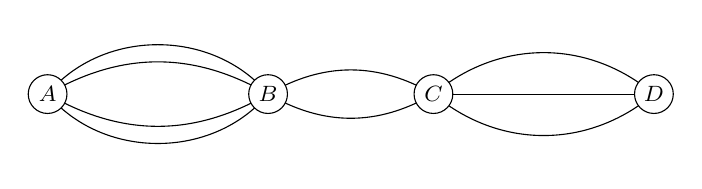
\begin{tikzpicture}[scale=0.7,font=\footnotesize, line join=round, line cap=round, >=stealth]
		\coordinate (A) at (0,0);
		\coordinate (B) at (4,0);
		\coordinate (C) at (7,0);
		\coordinate (D) at (11,0);
		\draw (A) to [out=-30, in=-150] (B);
		\draw (A) to [out=-50, in=-130] (B);
		\draw (A)to [out=30, in=150] (B) to [out=30, in=150] (C) to [out=40, in=140](D);
		\draw (A) to [out=50, in=130] (B) to [out=-30, in=-150] (C) to [out=-40, in=-140](D);
		\draw (C) to [out=0, in=180] (D);
		\draw[fill=white] 
		(A) node {$A$} circle (10pt)
		(B) node {$B$} circle (10pt)
		(C) node {$C$} circle (10pt)
		(D) node {$D$} circle (10pt);
	\end{tikzpicture}
\end{center}
Hỏi có bao nhiêu cách đi từ $A$ đến $D$ mà qua $B$ và $C$ chỉ một lần?
\choice
{$10$}
{$18$}
{$9$}
{\True $24$}
	\loigiai{
	Đi từ thành phố $A$ đến $B$ có $4$ cách đi.\\
	Đi từ thành phố $B$ đến $C$ có $2$ cách đi.\\
	Đi từ thành phố $C$ đến $D$ có $3$ cách đi.\\
	Theo quy tắc nhân, số cách đi từ $A$ đến $D$ là $4\cdot 3\cdot 2=24$ cách đi.
}
\end{ex}

\begin{ex}%[0X3Y2-4]%[Dự án đề kiểm tra HKII NH22-23 - Lê Hùng Thắng]%[THPT Trần Quốc Tuấn - Kon Tum]%Câu 30
Xét phép thử với không gian mẫu $\Omega$. Giả sử $A$ là một biến cố liên quan đến phép thử. Xác suất của biến cố $A$ là
\choice
{$ P(A)=\dfrac{n(\Omega)}{n(A)}$}
{$ P(A)=1-\dfrac{n(A)}{n(\Omega)}$}
{\True $ P(A)=\dfrac{n(A)}{n(\Omega)}$}
{$ P(A)=\dfrac{1-n(A)}{n(\Omega)}$}
\loigiai{
	Xác suất của biến cố $A$ là $ P(A)=\dfrac{n(A)}{n(\Omega)}$.
}
\end{ex}

\begin{ex}%[0X2Y2-2]%[Dự án đề kiểm tra HKII NH22-23 - Lê Hùng Thắng]%[THPT Trần Quốc Tuấn - Kon Tum]%Câu 31
Một tổ lao động gồm $10$ học sinh. Số cách chọn $4$ học sinh từ $10$ học sinh là
\choice
{$\mathrm{A}_{10}^4$}
{\True $\mathrm{C}_{10}^4$}
{$4^{10}$}
{$10^4$}
\loigiai{
	Số cách chọn $4$ học sinh từ $10$ học sinh là $\mathrm{C}_{10}^4$ cách.
}
\end{ex}

\begin{ex}%[0X2B2-2]%[Dự án đề kiểm tra HKII NH22-23 - Lê Hùng Thắng]%[THPT Trần Quốc Tuấn - Kon Tum]%Câu 32
Lớp 10C có $40$ học sinh trong đó có $18$ nam và $22$ nữ. Giáo viên chủ nhiệm cần chọn $3$ học sinh để trực an toàn giao thông gồm $2$ nam và $1$ nữ. Hỏi giáo viên chủ nhiệm có bao nhiêu cách chọn?
\choice
{$175$}
{$9880$}
{\True $3366$}
{$ 4158$}
\loigiai{
	Số cách chọn $2$ học sinh nam từ $18$ nam là $\mathrm{C}_{18}^2=153$ cách.\\
	Số cách chọn $1$ học sinh nữ từ $22$ nữ là $\mathrm{C}_{22}^1= 22$ cách.\\
Số cách chọn $3$ học sinh để trực an toàn giao thông gồm $2$ nam và $1$ nữ là $153\cdot 22=3366$ cách.
}
\end{ex}

\begin{ex}%[0H4Y2-2]%[Dự án đề kiểm tra HKII NH22-23 - Lê Hùng Thắng]%[THPT Trần Quốc Tuấn - Kon Tum]%Câu 33
Trong mặt phẳng $Oxy$, đường tròn có tâm là gốc tọa độ $O$ và bán kính $R$ có phương trình là
\choice
{$x^2+y^2=0$}
{\True $x^2+y^2=R^2$}
{$x^2-y^2=R^2$}
{$x^2+y^2=R$}
\loigiai{
	Đường tròn tâm $O$ và bán kính $R$ có phương trình là $x^2+y^2=R^2$.
}
\end{ex}

\begin{ex}%[0X1B4-3]%[Dự án đề kiểm tra HKII NH22-23 - Lê Hùng Thắng]%[THPT Trần Quốc Tuấn - Kon Tum]%Câu 34
Cho mẫu số liệu thống kê nhiệt độ (đơn vị: $^\circ C$) ở thị trấn Đăk Hà ngày $20/04/2023$ sau một số lần đo là: $ 21; \; 23; \; 25; \; 28; \; 30; \; 32; \; 34; \; 31; \; 29; \; 26$. Độ lệch chuẩn của mẫu số liệu đó gần nhất với kết quả nào sau đây?
\choice
{\True $3,91$}
{$4$}
{$3,8$}
{$3,9$}
\loigiai{
	Sử dụng máy tính cầm tay nhập số liệu và tính toán ta được kết quả độ lệch chuẩn của mẫu số liệu là $s\approx 3,91$.
}
\end{ex}

\begin{ex}%[0H4Y1-1]%[Dự án đề kiểm tra HKII NH22-23 - Lê Hùng Thắng]%[THPT Trần Quốc Tuấn - Kon Tum]%Câu 35
Trong mặt phẳng $Oxy$, cho đường thẳng $\Delta \colon \left\{\begin{aligned}
& x=-1+3t\\ & y=4-2t\\ \end{aligned}\right.$. Véc-tơ nào sau đây là véc-tơ chỉ phương của đường thẳng $\Delta$?
\choice
{$\overrightarrow{u}=(3;2)$}
{$\overrightarrow{u}=(-1;4)$}
{\True $\overrightarrow{u}=(3;-2)$}
{$\overrightarrow{u}=(-1;-2)$}
\loigiai{
	Đường thẳng $\Delta$ có véc-tơ chỉ phương là $\overrightarrow{u}=(3;-2)$.
}
\end{ex}

\Closesolutionfile{ans}
%\begin{center}
%	\textbf{ĐÁP ÁN}
%	\inputansbox{10}{ans/ans}	
%\end{center}
\begin{center}
	\textbf{PHẦN 2 - TỰ LUẬN}
\end{center}

\begin{bt}%[0X3B2-1]%[Dự án đề kiểm tra HKII NH22-23 - Lê Hùng Thắng]%[THPT Trần Quốc Tuấn - Kon Tum]%Câu 36
	Tung một đồng xu cân đối và đồng chất liên tiếp ba lần.
	\begin{enumEX}{1}
		\item Viết tập hợp $\Omega $ là không gian mẫu trong trò chơi trên.
		\item Tính xác suất của biến cố A: “Mặt sấp xuất hiện đúng hai lần”
	\end{enumEX}
	\loigiai{
	\begin{enumEX}{1}
		\item Không gian mẫu $\Omega=\left\{ SSS,SSN,SNS,NSS,SNN,NSN,NNS,NNN\right\}$.
		\item Số phần tử của không gian mẫu: $ n(\Omega)=8$.\\
		$ A=\{SSN,SNSN,NSS\}\Rightarrow n(A)=3$.\\
		Xác suất của biến cố A: $ P(A)=\dfrac{n(A)}{n(\Omega)}=\dfrac{3}{8}$.
	\end{enumEX}
	}
\end{bt}

\begin{bt}%[0H4B3-2]%[Dự án đề kiểm tra HKII NH22-23 - Lê Hùng Thắng]%[THPT Trần Quốc Tuấn - Kon Tum]%Câu 37
	Viết phương trình chính tắc của Elip, biết $(E)$ có một tiêu điểm $F_2(5;0)$ và đi qua điểm $M(0;3)$.
	\loigiai{
		Giả sử phương trình chính tắc của Elip có dạng $\dfrac{x^2}{a^2}+\dfrac{y^2}{b^2}=1$, $(a>b>0)$.\\
		Vì $(E)$ có một tiêu điểm $F_2(5;0)$ nên $ c=5$.\\
		Vì $(E)$ đi qua điểm $M(0;3)$ nên $\dfrac{0^2}{a^2}+\dfrac{3^2}{b^2}=1 \Rightarrow{b^2}=9$.\\
		Ta có $a^2=b^2+c^2=25+9=34$.\\
		Vậy phương trình chính tắc của $(E)$ là $\dfrac{x^2}{34}+\dfrac{y^2}{9}=1$.
	}
\end{bt}

\begin{bt}%[0H4K2-2]%[Dự án đề kiểm tra HKII NH22-23 - Lê Hùng Thắng]%[THPT Trần Quốc Tuấn - Kon Tum]%Câu 38
	Viết phương trình đường tròn $(C)$ có bán kính $R=2$, tâm $I$ thuộc đường thẳng $\Delta_1\colon \left\{\begin{aligned}
		& x=1+t\\ & y=1-t\\ \end{aligned}\right.$ và $(C)$ tiếp xúc với đường thẳng $\Delta_2\colon 3x+4y-1=0$.
	\loigiai{
	Theo đề $I\in \Delta_1\Rightarrow I(1+t;1-t)$.\\
	Vì $(C)$ tiếp xúc với đường thẳng $\Delta_2$ và có bán kính $R=2$ nên ta có\\
	\allowdisplaybreaks \vspace*{-0.7cm}
	\begin{eqnarray*} 
		& R= &\mathrm{d}(I,\Delta_2)=2\\ 
		& \Leftrightarrow & \dfrac{\left| 3(1+t)+4(1-t)-1\right|}{\sqrt{3^2+4^2}}=2\\ 
		& \Leftrightarrow & \left| 6-t\right|=10\\ 
		& \Leftrightarrow & \left[\begin{aligned}
			& t=-4\\ & t=16.\\ 
	\end{aligned}\right.
	\end{eqnarray*}
		Với $t=-4\Rightarrow I\left(-3;5\right)$; 
		và $t=16\Rightarrow I\left(17;-15\right)$.\\
		Vậy có hai đường tròn $(C)$ cần tìm là:\\ $\left(x+3\right)^2+\left(y-5\right)^2=4$
		hoặc $\left(x-17\right)^2+\left(y+15\right)^2=4$.
		}
\end{bt}

\begin{bt}%[0X3K2-6]%[Dự án đề kiểm tra HKII NH22-23 - Lê Hùng Thắng]%[THPT Trần Quốc Tuấn - Kon Tum]%Câu 39
	Gọi $S$ là tập hợp tất cả các số tự nhiên gồm hai chữ số khác nhau lập được từ các chữ số $\left\{0,1,2,3,4,5,6\right\}$. Chọn ngẫu nhiên hai số từ tập $S$. Tính xác suất để hai số lấy ra từ tập $S$ đều là số lẻ.
	\loigiai{
		Số phần tử của tập $S$ là $6\cdot 6=36$.\\
		Suy ra số phần tử của không gian mẫu là $n(\Omega)=\mathrm{C}_{36}^2$.\\
		Gọi biến cố $A\colon$“Hai số lấy ra đều là số lẻ”.\\
		Trong $36$ số của tập hợp $S$ có $15$ số lẻ và $21$ số chẵn.\\
		Do đó $n(A)=\mathrm{C}_{15}^2$.\\
		Xác suất của biến cố $A$ là $ P(A)=\dfrac{n(A)}{n(\Omega)}=\dfrac{\mathrm{C}_{15}^2}{\mathrm{C}_{36}^2}=\dfrac{1}{6}$.
		}
\end{bt}
